\documentclass[a4paper,12pt]{article}
\usepackage[utf8]{inputenc}
\usepackage[T1]{fontenc}
\usepackage[spanish]{babel}
\usepackage{csquotes}
\usepackage{hyperref}
\usepackage{anysize}
\usepackage{graphicx}
\marginsize{25mm}{25mm}{25mm}{25mm}

\title{Why do people gamble and keep gambling despite heavy losses?}
\author{Howard Rachlin}
\date{1990}

\begin{document}
{\scshape\bfseries \maketitle}

Un problema en conducta de juego es que no parece haber algo tangible ({\itshape commodity}) a lo cual ser adicto, a diferencia de las sustancias de abuso. No se puede decir que un apostador consuma dinero de la misma manera que un alcohólico consume alcohol.

Aunque los apostadores buscan el riesgo, el riesgo no es una {\itshape commodity}, sino un patrón de interacción con el ambiente---justamente lo que estudia el conductismo. Por lo tanto, el artículo pretende llevar el problema del juego al análisis de la conducta.

\section{Other theories}

Una explicación son los heurísticos ({\itshape e.g., disponibilidad}) mezclados con una motivación general para obtener dinero. Un problema con esta teoría es que no se especifican reglas que permitan determinar qué heurístico se aplicará a una situación particular, siendo que distintos heurísticos pueden llevar a comportamientos opuestos. Además, la explicación de sesgos y heurísticos no da atención a factores motivacionales: presume que todas las personas tienen la misma motivación para ganar pero los apostadores son menos racionales. Sin embargo, no hay evidencia que indique que de hecho sean menos racionales al juzgar resultados probabilísticos.

Esta teoría es similar a la del {\itshape prospecto}, según la cual primero se realiza un encuadre ({\itshape framing}, dar cuenta del contexto), y edición ({\itshape editing}, reestructurar alternativas), y después cada resultado posible se expresa como un producto de un {\slshape peso de decisión}, que es una función de la probabilidad $p$ del resultado y un {\slshape valor}, que es una función de la cantidad $A$ ganada o perdida para ese resultado.

El valor de la alternativa es la suma de los productos de los pesos de decisión y valores de todos los resultados contingentes a la elección de la alternativa. Dadas varias alternativas se elegirá aquella con el mayor valor general. Según la teoría, solo algunas personas apuestan dadas diferencias individuales en el encuadre y en las dos relaciones funcionales dichas.

Un problema con la teoría del prospecto es que su unidad fundamental es la apuesta única con resultados posibles fijos. En estudios de laboratorio las personas evitan el riesgo en alternativas de una sola ocasión, pero se ha encontrado que las preferencias se revierten cuando la misma alternativa se repite diez veces (más similar a las apuestas seriales de la conducta de juego).

La teoría presente, a diferencia de la teoría del prospecto, toma como unidad fundamental una serie de elecciones con un resultado fijo (y no una sola elección con varios resultados posibles). Al ver al juego como una serie de eventos en el tiempo, la demora se vuelve importante. La segunda diferencia con el prospecto es que da cuenta de la demora además de la probabilidad.

\section{The structure of a gamble}

Según Skinner una apuesta tiene la estructura de un programa de reforzamiento de razón variable (RV)---una serie de cadenas ({\itshape strings}) operantes que llevan al reforzamiento positivo.

Mowrer y Jones encontraron que el número de respuestas requisito de un programa se reflejaba en el número de respuestas emitidas en extinción, y especularon que las ratas emiten una cantidad de {\slshape unidades de respuesta} en extinción y no una cantidad dada de respuestas componentes. Esta unidad-de-respuesta es definida por las condiciones durante el reforzamiento.

El elemento probabilístico importante en esa visión no es el resultado de una respuesta dada, sino la longitud de la cadena de pérdidas que llevan a una ganancia. Para una probabilidad $p$ de una apuesta, la cantidad media de operantes en una cadena es $ \frac{1}{p}$ (el valor del programa de RV). La presunción clave es que la unidad conductual fundamental es la cadena: la pérdida individual no tiene valor negativo en tanto que es parte de una cadena y solo la cadena tiene valor; es decir, pérdidas y ganancias son sumadas solo al ganar al final de una cadena, y entonces el sistema se reinicia.

Por ejemplo, en apuestas de \$1 con probabilidad de .25 de ganar \$3, el valor esperado de la apuesta es cero ($3 \times \frac{1}{4} - 1 \times \frac{3}{4}$). Las 25 cadenas más probables de resultados (G, PG, PPG, PPPG, PPPPG, etc) llevan a un valor esperado de +2 centavos, por lo que, dado que el valor de la apuesta es cero, las cadenas 26 a infinito deben sumar -2 centavos. Esas últimas cadenas serán ignoradas.

\begin{figure}[!ht]
    \begin{center}
        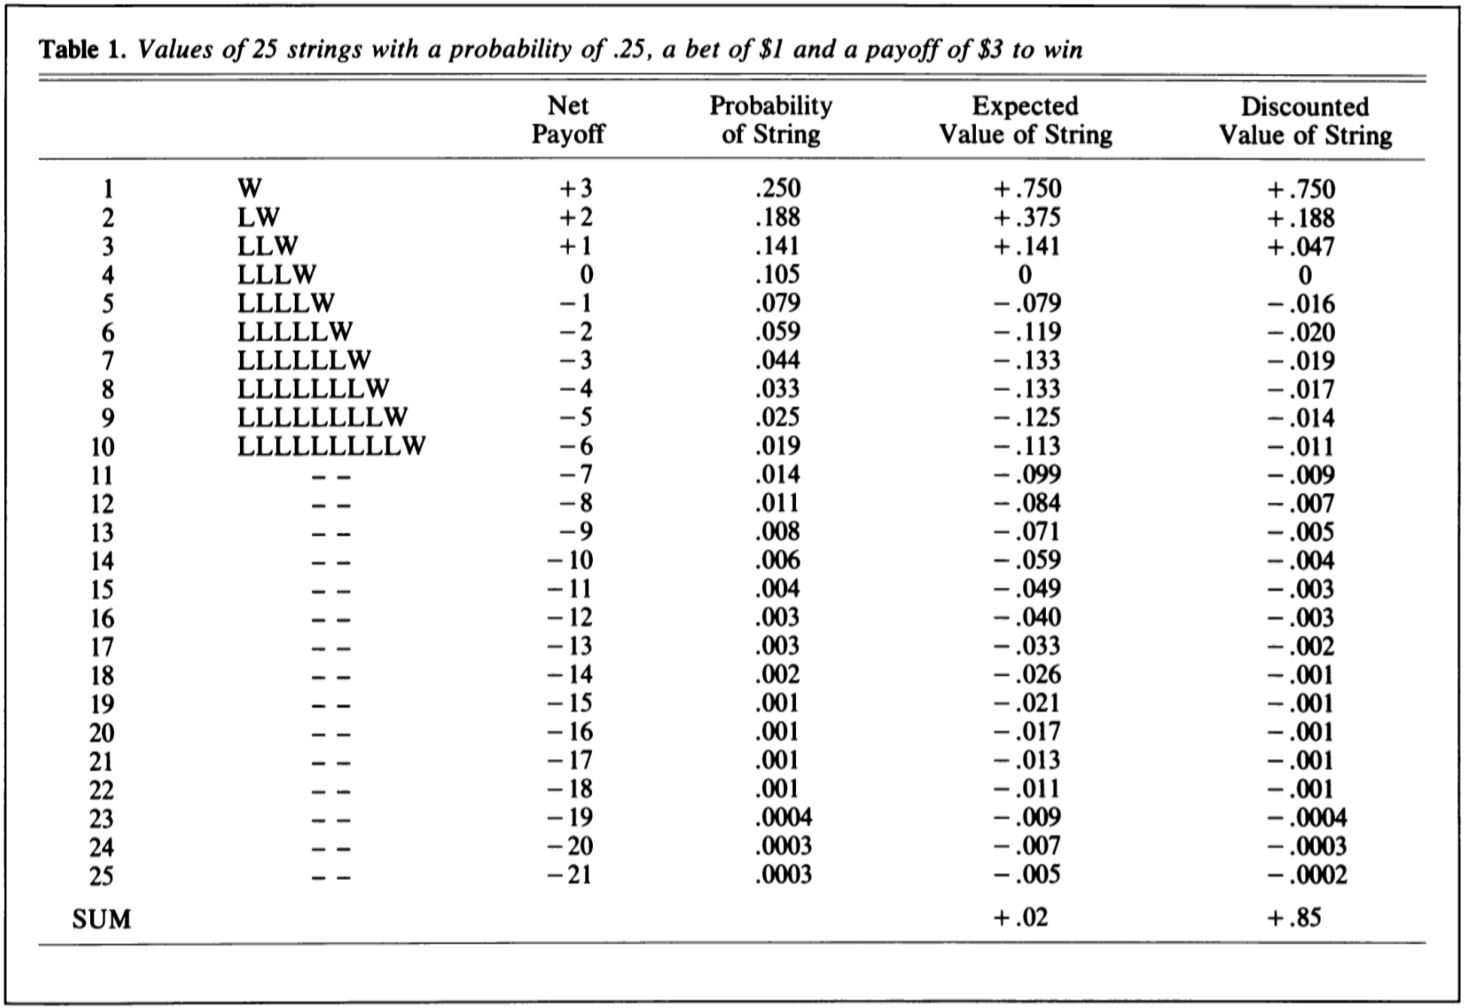
\includegraphics[scale=0.4]{Rachlin1990(1).png}
    \end{center}
\end{figure}

Las cadenas cortas son positivas, y las largas son negativas. Por lo tanto, para el apostador los resultados positivos ocurrirán pronto, y los negativos estarán demorados. Cuanto más positivo el resultado, más pronto se percibe que ocurrirá.

Se ha encontrado que los resultados demorados son descontados por la función hiperbólica
\begin{eqnarray}
    f(d) = \frac{1}{1 + kd}
\end{eqnarray}
donde $d$ es la demora, y $k$ es una constante que refleja la tasa de descuento. Según la teoría del prospecto el valor de la apuesta es una función de probabilidad, $g(p)$, multiplicada por una función de la cantidad, $h(A)$. Considerando cadenas con distintas demoras como unidades, el valor de una cadena es 
\begin{eqnarray}
    v = f(d)g(p)h(A)
\end{eqnarray}
Supóngase que $g(p)$ es igual a $p$, $h(A)$ es igual a $A$, $f(d)$ es igual al valor dado por la ecuación 1, la tasa de descuento $k$ es igual a 1, y el resultado de la primera cadena tiene $d = 0$. Con el valor descontado de cada una de las 25 cadenas consideradas la suma sería ahora de +85 centavos. Según incrementa la tasa de descuento de $k = 0 $ el valor positivo de la apuesta incrementa a un máximo y luego decrementa a una asíntota igual al valor de la primera cadena sin demora. Todas las otras cadenas serían eventualmente 100\% descontadas. Para el ejemplo dado, la asíntota sería de +75 centavos. Si $k$ estuviese inicialmente por encima del punto de máximo valor, decrementos en el grado de descuento $k$ llevarían a incrementos en el valor subjetivo de la apuesta.

Según esta explicación lo que da valor a las apuestas es el modo de estructuración y conteo de la apuesta---sumar ganancias y pérdidas al final de las cadenas---, y no el grado de descuento. Una apuesta como la considerada, con valor esperado de cero, solo sería valorada objetivamente si los eventos no fuesen descontados en absoluto ($k = 0$).

Este modelo explicaría la participación en lotería igual que en otras apuestas, aunque en ese caso las personas que nunca ganan nunca hacen un ajuste de cuentas. No se consideran las pérdidas porque siempre serían sobrepasadas por una ganancia eventual. Para una apuesta de valor esperado constante, incremento en la probabilidad de ganar (por lo tanto, decremento en la cantidad ganada) disminuye la cantidad de cadenas positivas antes de llegar a una negativa. Para la apuesta de la tabla hay tres cadenas positivas. Si la probabilidad de ganar fuera 0.5 habría solo 1, y en las loterías hay una cantidad virtualmente infinita de cadenas positivas.

\section{Altering strings}

Tras una serie suficientemente larga de pérdidas una ganancia no es ya redituable. Una manera de compensar sería incrementar la apuesta por una más riesgosa, con menos probabilidad de éxito pero con más ganancia, de manera tal que la cadena completa resulte en positivo. Si la cadena es la unidad básica, entonces los apostadores deberían tender a incrementar el riesgo tras perder, y se ha encontrado evidencia de ello en jugadores de ruleta y en apostadores en carreras.

El caso es similar al caso del ``costo hundido''. Cuanto más se deba esperar por la recompensa, más grande debe ser esta para justificar la espera y las pérdidas.

Lo anterior puede explicar por qué las personas comienzan a apostar, pero no por qué persisten a pesar de las pérdidas. ¿Por qué las personas no ajustan sus apuestas ante grandes cadenas de pérdidas?

\section{Compulsive gambling}

Las diferencias en la capacidad de demorar la gratificación pueden caracterizarse en términos de descuento temporal (niños pequeños podrían descontar más abruptamente las recompensas), o en términos de la extensión y complejidad de la estructura conductual (los niños pueden no ser capaces de organizar su conducta en cadenas de gran duración, y por lo tanto se pierden las ganancias a largo plazo).

Se puede decir, si estas hipótesis son válidas, que los adultos aprenden a controlarse mediante la acción de mecanismos internos que sirven para (a) decrementar el descuento temporal $k$ o (b) incrementar la extensión temporal de la unidad conductual. Sin embargo, este análisis sugiere que ningún mecanismo que cumpla esos fines disminuirá las apuestas compulsivas. La reducción de $k$, salvo a valores irrealmente bajos, incrementaría el valor subjetivo de las apuestas. Y dada la naturaleza estocástica de las apuestas incrementar el tamaño de la unidad de respuesta solo empeoraría el problema.

Ciertos mecanismos podrían mantener las apuestas bajo control. Si las unidades conductuales fuesen números fijos de apuestas o de tiempo, y si se hicieran cuentas tras cada unidad, las unidades positivas no ocurrirían más pronto que las negativas. Sin embargo, con programas de RV la señal que indica el final de una unidad (una ganancia) es intrínseca a la actividad misma. Reestructurar para tomar en cuenta un conteo o tiempo requeriría señales no provistas en la situación de apuesta.

La expansión gradual del requisito de respuesta en programas RV en el laboratorio ha llevado a soportar cientos o miles de respuestas sin reforzamiento. Una historia similar podría caracterizar a los apostadores compulsivos. Para ellos, reestructurar con base en conteo o tiempo podría ser especialmente difícil.


\end{document}
